\documentclass[]{article}
\usepackage{lmodern}
\usepackage{amssymb,amsmath}
\usepackage{ifxetex,ifluatex}
\usepackage{fixltx2e} % provides \textsubscript
\ifnum 0\ifxetex 1\fi\ifluatex 1\fi=0 % if pdftex
  \usepackage[T1]{fontenc}
  \usepackage[utf8]{inputenc}
\else % if luatex or xelatex
  \ifxetex
    \usepackage{mathspec}
  \else
    \usepackage{fontspec}
  \fi
  \defaultfontfeatures{Ligatures=TeX,Scale=MatchLowercase}
\fi
% use upquote if available, for straight quotes in verbatim environments
\IfFileExists{upquote.sty}{\usepackage{upquote}}{}
% use microtype if available
\IfFileExists{microtype.sty}{%
\usepackage{microtype}
\UseMicrotypeSet[protrusion]{basicmath} % disable protrusion for tt fonts
}{}
\usepackage[margin=1in]{geometry}
\usepackage{hyperref}
\hypersetup{unicode=true,
            pdftitle={SL Homework 5},
            pdfauthor={Joshua Ingram},
            pdfborder={0 0 0},
            breaklinks=true}
\urlstyle{same}  % don't use monospace font for urls
\usepackage{color}
\usepackage{fancyvrb}
\newcommand{\VerbBar}{|}
\newcommand{\VERB}{\Verb[commandchars=\\\{\}]}
\DefineVerbatimEnvironment{Highlighting}{Verbatim}{commandchars=\\\{\}}
% Add ',fontsize=\small' for more characters per line
\usepackage{framed}
\definecolor{shadecolor}{RGB}{248,248,248}
\newenvironment{Shaded}{\begin{snugshade}}{\end{snugshade}}
\newcommand{\AlertTok}[1]{\textcolor[rgb]{0.94,0.16,0.16}{#1}}
\newcommand{\AnnotationTok}[1]{\textcolor[rgb]{0.56,0.35,0.01}{\textbf{\textit{#1}}}}
\newcommand{\AttributeTok}[1]{\textcolor[rgb]{0.77,0.63,0.00}{#1}}
\newcommand{\BaseNTok}[1]{\textcolor[rgb]{0.00,0.00,0.81}{#1}}
\newcommand{\BuiltInTok}[1]{#1}
\newcommand{\CharTok}[1]{\textcolor[rgb]{0.31,0.60,0.02}{#1}}
\newcommand{\CommentTok}[1]{\textcolor[rgb]{0.56,0.35,0.01}{\textit{#1}}}
\newcommand{\CommentVarTok}[1]{\textcolor[rgb]{0.56,0.35,0.01}{\textbf{\textit{#1}}}}
\newcommand{\ConstantTok}[1]{\textcolor[rgb]{0.00,0.00,0.00}{#1}}
\newcommand{\ControlFlowTok}[1]{\textcolor[rgb]{0.13,0.29,0.53}{\textbf{#1}}}
\newcommand{\DataTypeTok}[1]{\textcolor[rgb]{0.13,0.29,0.53}{#1}}
\newcommand{\DecValTok}[1]{\textcolor[rgb]{0.00,0.00,0.81}{#1}}
\newcommand{\DocumentationTok}[1]{\textcolor[rgb]{0.56,0.35,0.01}{\textbf{\textit{#1}}}}
\newcommand{\ErrorTok}[1]{\textcolor[rgb]{0.64,0.00,0.00}{\textbf{#1}}}
\newcommand{\ExtensionTok}[1]{#1}
\newcommand{\FloatTok}[1]{\textcolor[rgb]{0.00,0.00,0.81}{#1}}
\newcommand{\FunctionTok}[1]{\textcolor[rgb]{0.00,0.00,0.00}{#1}}
\newcommand{\ImportTok}[1]{#1}
\newcommand{\InformationTok}[1]{\textcolor[rgb]{0.56,0.35,0.01}{\textbf{\textit{#1}}}}
\newcommand{\KeywordTok}[1]{\textcolor[rgb]{0.13,0.29,0.53}{\textbf{#1}}}
\newcommand{\NormalTok}[1]{#1}
\newcommand{\OperatorTok}[1]{\textcolor[rgb]{0.81,0.36,0.00}{\textbf{#1}}}
\newcommand{\OtherTok}[1]{\textcolor[rgb]{0.56,0.35,0.01}{#1}}
\newcommand{\PreprocessorTok}[1]{\textcolor[rgb]{0.56,0.35,0.01}{\textit{#1}}}
\newcommand{\RegionMarkerTok}[1]{#1}
\newcommand{\SpecialCharTok}[1]{\textcolor[rgb]{0.00,0.00,0.00}{#1}}
\newcommand{\SpecialStringTok}[1]{\textcolor[rgb]{0.31,0.60,0.02}{#1}}
\newcommand{\StringTok}[1]{\textcolor[rgb]{0.31,0.60,0.02}{#1}}
\newcommand{\VariableTok}[1]{\textcolor[rgb]{0.00,0.00,0.00}{#1}}
\newcommand{\VerbatimStringTok}[1]{\textcolor[rgb]{0.31,0.60,0.02}{#1}}
\newcommand{\WarningTok}[1]{\textcolor[rgb]{0.56,0.35,0.01}{\textbf{\textit{#1}}}}
\usepackage{graphicx,grffile}
\makeatletter
\def\maxwidth{\ifdim\Gin@nat@width>\linewidth\linewidth\else\Gin@nat@width\fi}
\def\maxheight{\ifdim\Gin@nat@height>\textheight\textheight\else\Gin@nat@height\fi}
\makeatother
% Scale images if necessary, so that they will not overflow the page
% margins by default, and it is still possible to overwrite the defaults
% using explicit options in \includegraphics[width, height, ...]{}
\setkeys{Gin}{width=\maxwidth,height=\maxheight,keepaspectratio}
\IfFileExists{parskip.sty}{%
\usepackage{parskip}
}{% else
\setlength{\parindent}{0pt}
\setlength{\parskip}{6pt plus 2pt minus 1pt}
}
\setlength{\emergencystretch}{3em}  % prevent overfull lines
\providecommand{\tightlist}{%
  \setlength{\itemsep}{0pt}\setlength{\parskip}{0pt}}
\setcounter{secnumdepth}{0}
% Redefines (sub)paragraphs to behave more like sections
\ifx\paragraph\undefined\else
\let\oldparagraph\paragraph
\renewcommand{\paragraph}[1]{\oldparagraph{#1}\mbox{}}
\fi
\ifx\subparagraph\undefined\else
\let\oldsubparagraph\subparagraph
\renewcommand{\subparagraph}[1]{\oldsubparagraph{#1}\mbox{}}
\fi

%%% Use protect on footnotes to avoid problems with footnotes in titles
\let\rmarkdownfootnote\footnote%
\def\footnote{\protect\rmarkdownfootnote}

%%% Change title format to be more compact
\usepackage{titling}

% Create subtitle command for use in maketitle
\providecommand{\subtitle}[1]{
  \posttitle{
    \begin{center}\large#1\end{center}
    }
}

\setlength{\droptitle}{-2em}

  \title{SL Homework 5}
    \pretitle{\vspace{\droptitle}\centering\huge}
  \posttitle{\par}
    \author{Joshua Ingram}
    \preauthor{\centering\large\emph}
  \postauthor{\par}
      \predate{\centering\large\emph}
  \postdate{\par}
    \date{10/27/2019}


\begin{document}
\maketitle

\hypertarget{problem-1}{%
\subsection{Problem 1}\label{problem-1}}

\hypertarget{section}{%
\subsubsection{1.}\label{section}}

\(Sales = \beta_0 + \beta_1TV + (\beta_2 + \beta_3TV)radio + \epsilon\)

\hypertarget{section-1}{%
\subsubsection{2.}\label{section-1}}

\begin{Shaded}
\begin{Highlighting}[]
\KeywordTok{lm}\NormalTok{(Balance }\OperatorTok{~}\StringTok{ }\KeywordTok{I}\NormalTok{(Ethnicity }\OperatorTok{==}\StringTok{ "Asian"}\NormalTok{) }\OperatorTok{+}\StringTok{ }\KeywordTok{I}\NormalTok{(Ethnicity }\OperatorTok{==}\StringTok{ "Caucasian"}\NormalTok{) }\OperatorTok{+}\StringTok{ }\KeywordTok{I}\NormalTok{(Ethnicity }\OperatorTok{==}\StringTok{ "African - American"}\NormalTok{), }\DataTypeTok{data =}\NormalTok{ Credit)}
\end{Highlighting}
\end{Shaded}

\begin{verbatim}
## 
## Call:
## lm(formula = Balance ~ I(Ethnicity == "Asian") + I(Ethnicity == 
##     "Caucasian") + I(Ethnicity == "African - American"), data = Credit)
## 
## Coefficients:
##                              (Intercept)  
##                                   531.00  
##              I(Ethnicity == "Asian")TRUE  
##                                   -18.69  
##          I(Ethnicity == "Caucasian")TRUE  
##                                   -12.50  
## I(Ethnicity == "African - American")TRUE  
##                                       NA
\end{verbatim}

We recieve ``NA'' for our ``African-American'' dummy variable because we
are fitting a linear model using a categorical explanatory variable with
3 levels, but using 3 dummy variables. Instead, we should be using 2
dummy variables (K-1 categories) and using one of our levels as a
baseline category.

\hypertarget{section-2}{%
\subsubsection{3.}\label{section-2}}

\begin{Shaded}
\begin{Highlighting}[]
\KeywordTok{plot}\NormalTok{(mpg }\OperatorTok{~}\StringTok{ }\NormalTok{horsepower, }\DataTypeTok{data =}\NormalTok{ Auto)}
\NormalTok{x.grid <-}\StringTok{ }\KeywordTok{seq}\NormalTok{(}\KeywordTok{min}\NormalTok{(Auto}\OperatorTok{$}\NormalTok{horsepower), }\KeywordTok{max}\NormalTok{(Auto}\OperatorTok{$}\NormalTok{horsepower), }\DataTypeTok{length =} \DecValTok{100}\NormalTok{)}
\ControlFlowTok{for}\NormalTok{ (i }\ControlFlowTok{in} \DecValTok{1}\OperatorTok{:}\DecValTok{10}\NormalTok{)\{}
\NormalTok{  lm.fit <-}\StringTok{ }\KeywordTok{lm}\NormalTok{(mpg }\OperatorTok{~}\StringTok{ }\KeywordTok{poly}\NormalTok{(horsepower, i), }\DataTypeTok{data =}\NormalTok{ Auto)}
  \KeywordTok{lines}\NormalTok{(}\DataTypeTok{x=}\NormalTok{x.grid,}\DataTypeTok{y=}\KeywordTok{predict}\NormalTok{(lm.fit, }\DataTypeTok{newdata=}\KeywordTok{data.frame}\NormalTok{(}\DataTypeTok{horsepower=}\NormalTok{x.grid)), }\DataTypeTok{col =}\NormalTok{ i, }\DataTypeTok{lwd=}\FloatTok{1.5}\NormalTok{)}
\NormalTok{\}}
\end{Highlighting}
\end{Shaded}

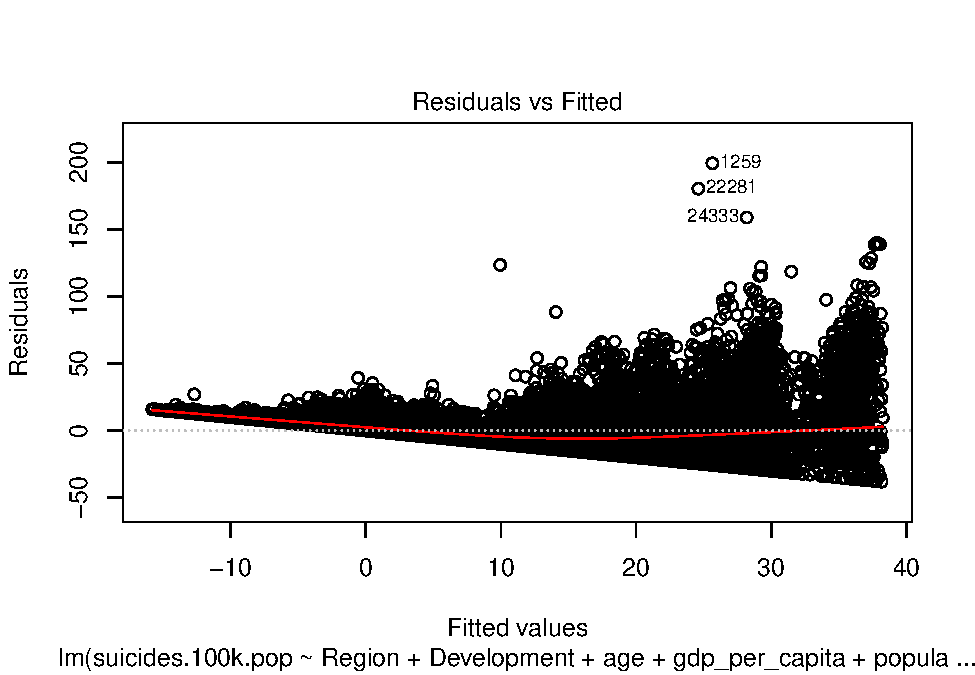
\includegraphics{SL_HW_5_files/figure-latex/unnamed-chunk-2-1.pdf}

\hypertarget{problem-2}{%
\subsection{Problem 2}\label{problem-2}}

\hypertarget{model-without-rv-and-weight}{%
\subsubsection{Model without rv and
weight}\label{model-without-rv-and-weight}}

\begin{Shaded}
\begin{Highlighting}[]
\NormalTok{lm.rv <-}\StringTok{ }\KeywordTok{lm}\NormalTok{(pemax }\OperatorTok{~}\StringTok{ }\NormalTok{sex }\OperatorTok{+}\StringTok{ }\NormalTok{height }\OperatorTok{+}\StringTok{ }\NormalTok{frc, }\DataTypeTok{data =}\NormalTok{ cystfibr)}
\KeywordTok{summary}\NormalTok{(lm.rv)}
\end{Highlighting}
\end{Shaded}

\begin{verbatim}
## 
## Call:
## lm(formula = pemax ~ sex + height + frc, data = cystfibr)
## 
## Residuals:
##     Min      1Q  Median      3Q     Max 
## -48.711 -21.067  -0.775  20.233  57.418 
## 
## Coefficients:
##              Estimate Std. Error t value Pr(>|t|)  
## (Intercept)  -7.88727   71.05326  -0.111   0.9127  
## sex         -12.53064   11.40646  -1.099   0.2844  
## height        0.83769    0.33821   2.477   0.0218 *
## frc          -0.03525    0.16681  -0.211   0.8347  
## ---
## Signif. codes:  0 '***' 0.001 '**' 0.01 '*' 0.05 '.' 0.1 ' ' 1
## 
## Residual standard error: 27.76 on 21 degrees of freedom
## Multiple R-squared:  0.3968, Adjusted R-squared:  0.3106 
## F-statistic: 4.604 on 3 and 21 DF,  p-value: 0.01255
\end{verbatim}

\hypertarget{model-with-rv-and-weight}{%
\subsubsection{Model with rv and
weight}\label{model-with-rv-and-weight}}

\begin{Shaded}
\begin{Highlighting}[]
\NormalTok{lm.rv <-}\StringTok{ }\KeywordTok{lm}\NormalTok{(pemax }\OperatorTok{~}\StringTok{ }\NormalTok{sex }\OperatorTok{+}\StringTok{ }\NormalTok{height }\OperatorTok{+}\StringTok{ }\NormalTok{frc }\OperatorTok{+}\StringTok{ }\NormalTok{weight }\OperatorTok{+}\StringTok{ }\NormalTok{rv, }\DataTypeTok{data =}\NormalTok{ cystfibr)}
\KeywordTok{summary}\NormalTok{(lm.rv)}
\end{Highlighting}
\end{Shaded}

\begin{verbatim}
## 
## Call:
## lm(formula = pemax ~ sex + height + frc + weight + rv, data = cystfibr)
## 
## Residuals:
##    Min     1Q Median     3Q    Max 
## -48.28 -19.82   0.91  15.83  37.97 
## 
## Coefficients:
##             Estimate Std. Error t value Pr(>|t|)  
## (Intercept) 104.4139    88.0781   1.185   0.2504  
## sex         -16.6162    11.0070  -1.510   0.1476  
## height       -0.2659     0.6775  -0.392   0.6991  
## frc          -0.5492     0.3231  -1.700   0.1055  
## weight        1.5027     0.8211   1.830   0.0830 .
## rv            0.3145     0.1648   1.909   0.0715 .
## ---
## Signif. codes:  0 '***' 0.001 '**' 0.01 '*' 0.05 '.' 0.1 ' ' 1
## 
## Residual standard error: 25.89 on 19 degrees of freedom
## Multiple R-squared:  0.5254, Adjusted R-squared:  0.4005 
## F-statistic: 4.207 on 5 and 19 DF,  p-value: 0.00963
\end{verbatim}

\hypertarget{a.}{%
\subsubsection{a.}\label{a.}}

The SE of frc is .16681 and the SE of height is .33821 in the model
without rv and weight, whereas the SE for frc and height are .3231 and
.6775, respectively. The SE for both variables increase when more
variables are introduced into the model, which suggests that there is
collinearity between the variables introduced and frc and height. This
is because we have more uncertainty when determining the effects of
these varaibles (which collinearity causes).

\hypertarget{b.}{%
\subsubsection{b.}\label{b.}}

\begin{Shaded}
\begin{Highlighting}[]
\KeywordTok{vif}\NormalTok{(}\KeywordTok{lm}\NormalTok{(pemax }\OperatorTok{~}\NormalTok{., }\DataTypeTok{data =}\NormalTok{ cystfibr))}
\end{Highlighting}
\end{Shaded}

\begin{verbatim}
##       age       sex    height    weight       bmp      fev1        rv 
## 21.829841  2.269407 13.954929 47.781303  7.115752  5.419507 10.538052 
##       frc       tlc 
## 17.143073  2.659993
\end{verbatim}

\begin{Shaded}
\begin{Highlighting}[]
\CommentTok{# remove weight as it has highest VIF}
\KeywordTok{vif}\NormalTok{(}\KeywordTok{lm}\NormalTok{(pemax}\OperatorTok{~}\NormalTok{.}\OperatorTok{-}\NormalTok{weight, }\DataTypeTok{data =}\NormalTok{  cystfibr))}
\end{Highlighting}
\end{Shaded}

\begin{verbatim}
##       age       sex    height       bmp      fev1        rv       frc 
##  8.097571  2.029182  7.595539  2.730462  4.205260 10.332505 15.814231 
##       tlc 
##  2.177076
\end{verbatim}

\begin{Shaded}
\begin{Highlighting}[]
\CommentTok{# remove frc as it has highest VIF}
\KeywordTok{vif}\NormalTok{(}\KeywordTok{lm}\NormalTok{(pemax }\OperatorTok{~}\StringTok{ }\NormalTok{.}\OperatorTok{-}\NormalTok{weight}\OperatorTok{-}\NormalTok{frc, }\DataTypeTok{data =}\NormalTok{ cystfibr))}
\end{Highlighting}
\end{Shaded}

\begin{verbatim}
##      age      sex   height      bmp     fev1       rv      tlc 
## 7.341695 1.606561 7.595520 1.794168 2.870202 2.836471 1.768577
\end{verbatim}

\begin{Shaded}
\begin{Highlighting}[]
\CommentTok{# remove height because it has highest VIF, still above 5}
\KeywordTok{vif}\NormalTok{(}\KeywordTok{lm}\NormalTok{(pemax }\OperatorTok{~}\StringTok{ }\NormalTok{.}\OperatorTok{-}\NormalTok{weight}\OperatorTok{-}\NormalTok{frc}\OperatorTok{-}\NormalTok{height, }\DataTypeTok{data =}\NormalTok{ cystfibr))}
\end{Highlighting}
\end{Shaded}

\begin{verbatim}
##      age      sex      bmp     fev1       rv      tlc 
## 1.611582 1.605444 1.718765 2.861478 2.814628 1.768466
\end{verbatim}

First weight is dropped, second frc, followed by height. This is our
simplified model that removes any variables with collinearity (or
multi-collinearity), which is why we used VIF, so that we could check
for any of this. The three removed variables had some relationship with
other variables within the model.

\hypertarget{problem-3}{%
\subsection{Problem 3}\label{problem-3}}

\hypertarget{a.-1}{%
\subsubsection{a.}\label{a.-1}}

\(\hat{\text{Starting Salary}}\) =
\(50 + 20(GPA) + 0.07(IQ) - 5(Gender) + 0.01(GPA*IQ) - 10(GPA*Gender)\)

\hypertarget{b.-1}{%
\subsubsection{b.}\label{b.-1}}

With all other variables held constant, we expect to see, on average,
that males will make \$5,000 more than females for starting salary.

\hypertarget{c.}{%
\subsubsection{c.}\label{c.}}

Based on our model, if we observe someone is female, we expecct to see,
on average, a ``decrease'' in starting salary by 5 + 10GPA (convert to
thousands of dollars). The effect of being female will also be dependent
upon GPA.

\hypertarget{d.}{%
\subsubsection{d.}\label{d.}}

With all other variables held constant, we expect, on average, to see an
increase in starting salary by \$70 for every one point increase in IQ.

\hypertarget{e.}{%
\subsubsection{e.}\label{e.}}

We expect to see, on average, an increase in starting salary by 0.07 +
0.01GPA (in thousands of dollars) for every one point increase in IQ.
The size of the effect of IQ on starting salary is dependent on GPA.

\hypertarget{f.}{%
\subsubsection{f.}\label{f.}}

\begin{Shaded}
\begin{Highlighting}[]
\NormalTok{prediction =}\StringTok{ }\DecValTok{50} \OperatorTok{+}\StringTok{ }\DecValTok{20}\OperatorTok{*}\DecValTok{4} \OperatorTok{+}\StringTok{ }\FloatTok{0.07}\OperatorTok{*}\DecValTok{110} \OperatorTok{-}\StringTok{ }\DecValTok{5}\OperatorTok{*}\DecValTok{1} \OperatorTok{+}\StringTok{ }\FloatTok{0.01}\OperatorTok{*}\NormalTok{(}\DecValTok{4}\OperatorTok{*}\DecValTok{110}\NormalTok{) }\OperatorTok{-}\StringTok{ }\DecValTok{10}\OperatorTok{*}\NormalTok{(}\DecValTok{4}\OperatorTok{*}\DecValTok{1}\NormalTok{)}
\NormalTok{prediction}
\end{Highlighting}
\end{Shaded}

\begin{verbatim}
## [1] 97.1
\end{verbatim}

We predict the starting salary to be \$97,100.

\hypertarget{g.}{%
\subsubsection{g.}\label{g.}}

False. The evidence for an interaction effect would be seen in the
p-value, not the size of the coefficient. There could be significant
evidence for a very small interaction effect between two variables, or
very little evidence for a very large interaction effect.

\hypertarget{problem-4}{%
\subsection{Problem 4}\label{problem-4}}

\hypertarget{section-3}{%
\subsubsection{1.}\label{section-3}}

\begin{Shaded}
\begin{Highlighting}[]
\NormalTok{lm.obj <-}\StringTok{ }\KeywordTok{lm}\NormalTok{(Sales }\OperatorTok{~}\StringTok{ }\NormalTok{Income }\OperatorTok{+}\StringTok{ }\NormalTok{Advertising }\OperatorTok{+}\StringTok{ }\NormalTok{ShelveLoc }\OperatorTok{+}\StringTok{ }\NormalTok{Urban, }\DataTypeTok{data =}\NormalTok{ Carseats)}
\KeywordTok{summary}\NormalTok{(lm.obj)}
\end{Highlighting}
\end{Shaded}

\begin{verbatim}
## 
## Call:
## lm(formula = Sales ~ Income + Advertising + ShelveLoc + Urban, 
##     data = Carseats)
## 
## Residuals:
##     Min      1Q  Median      3Q     Max 
## -6.6178 -1.5492  0.0182  1.4956  6.2868 
## 
## Coefficients:
##                 Estimate Std. Error t value Pr(>|t|)    
## (Intercept)     3.696673   0.411685   8.979  < 2e-16 ***
## Income          0.016499   0.003958   4.169 3.77e-05 ***
## Advertising     0.096308   0.016650   5.784 1.49e-08 ***
## ShelveLocGood   4.656799   0.329846  14.118  < 2e-16 ***
## ShelveLocMedium 1.837221   0.270946   6.781 4.39e-11 ***
## UrbanYes        0.045990   0.242571   0.190     0.85    
## ---
## Signif. codes:  0 '***' 0.001 '**' 0.01 '*' 0.05 '.' 0.1 ' ' 1
## 
## Residual standard error: 2.202 on 394 degrees of freedom
## Multiple R-squared:  0.3999, Adjusted R-squared:  0.3923 
## F-statistic: 52.51 on 5 and 394 DF,  p-value: < 2.2e-16
\end{verbatim}

\begin{Shaded}
\begin{Highlighting}[]
\KeywordTok{plot}\NormalTok{(lm.obj, }\DecValTok{1}\NormalTok{)}
\end{Highlighting}
\end{Shaded}

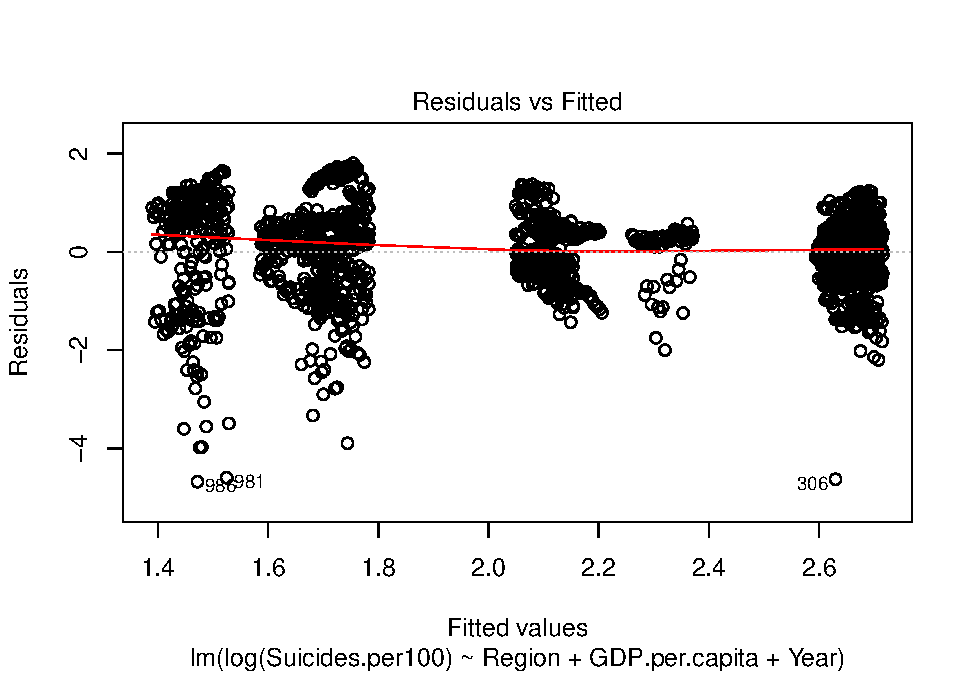
\includegraphics{SL_HW_5_files/figure-latex/unnamed-chunk-7-1.pdf}

Based on the residuals vs fitted plot, this seems like a good model to
use. This is because the variance of the residuals is pretty constant
throughout and there does not seem to be an odd shape or trend around
the 0.

The ShelvLoc variable is a categorical variable with three levels, good,
bad, and medium. By looking at documentation, it seems to deal with the
placement of the carseat in the store. Based on our model, we expect to
see sales increase, on average, by 4.66 units, with respect to ``bad''
ShelveLoc value, when ShelveLoc is ``Good'', where as we will see only
an increase of 1.84 when ShelveLoc is ``Medium'', with all other
variables held constant.

\hypertarget{section-4}{%
\subsubsection{2.}\label{section-4}}

\begin{Shaded}
\begin{Highlighting}[]
\NormalTok{lm.obj1 <-}\StringTok{ }\KeywordTok{lm}\NormalTok{(medv }\OperatorTok{~}\StringTok{ }\NormalTok{crim }\OperatorTok{+}\StringTok{ }\NormalTok{rm }\OperatorTok{+}\StringTok{ }\NormalTok{lstat, }\DataTypeTok{data =}\NormalTok{ Boston)}
\KeywordTok{summary}\NormalTok{(lm.obj1)}
\end{Highlighting}
\end{Shaded}

\begin{verbatim}
## 
## Call:
## lm(formula = medv ~ crim + rm + lstat, data = Boston)
## 
## Residuals:
##     Min      1Q  Median      3Q     Max 
## -17.925  -3.566  -1.157   1.906  29.024 
## 
## Coefficients:
##             Estimate Std. Error t value Pr(>|t|)    
## (Intercept) -2.56225    3.16602  -0.809  0.41873    
## crim        -0.10294    0.03202  -3.215  0.00139 ** 
## rm           5.21695    0.44203  11.802  < 2e-16 ***
## lstat       -0.57849    0.04767 -12.135  < 2e-16 ***
## ---
## Signif. codes:  0 '***' 0.001 '**' 0.01 '*' 0.05 '.' 0.1 ' ' 1
## 
## Residual standard error: 5.49 on 502 degrees of freedom
## Multiple R-squared:  0.6459, Adjusted R-squared:  0.6437 
## F-statistic: 305.2 on 3 and 502 DF,  p-value: < 2.2e-16
\end{verbatim}

\begin{Shaded}
\begin{Highlighting}[]
\KeywordTok{plot}\NormalTok{(lm.obj1, }\DecValTok{1}\NormalTok{)}
\end{Highlighting}
\end{Shaded}

\includegraphics{SL_HW_5_files/figure-latex/unnamed-chunk-8-1.pdf}

This model is not a good fit for the data, as the residuals follow a
non-linear trend.

\begin{Shaded}
\begin{Highlighting}[]
\KeywordTok{plot}\NormalTok{(medv }\OperatorTok{~}\StringTok{ }\NormalTok{crim, }\DataTypeTok{data =}\NormalTok{ Boston)}
\end{Highlighting}
\end{Shaded}

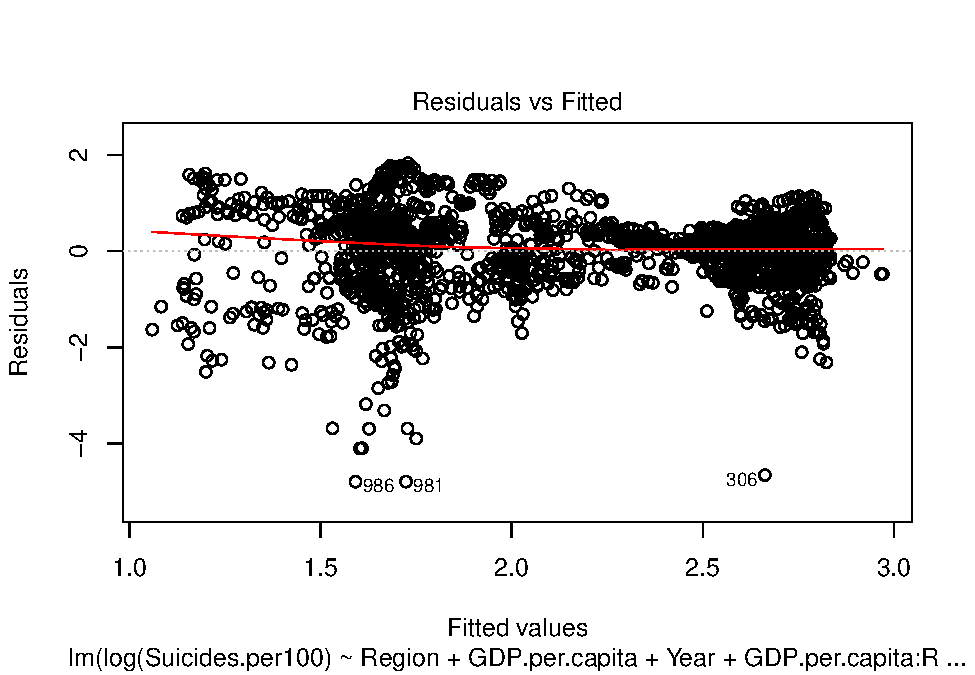
\includegraphics{SL_HW_5_files/figure-latex/unnamed-chunk-9-1.pdf}

\begin{Shaded}
\begin{Highlighting}[]
\KeywordTok{plot}\NormalTok{(medv }\OperatorTok{~}\StringTok{ }\NormalTok{rm, }\DataTypeTok{data =}\NormalTok{ Boston)}
\end{Highlighting}
\end{Shaded}

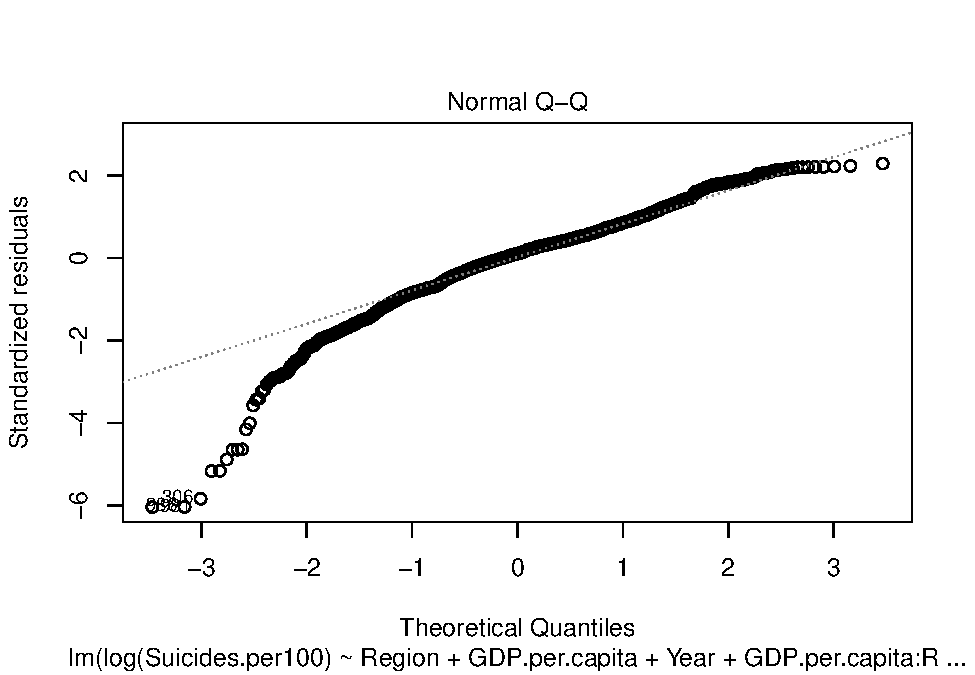
\includegraphics{SL_HW_5_files/figure-latex/unnamed-chunk-9-2.pdf}

\begin{Shaded}
\begin{Highlighting}[]
\KeywordTok{plot}\NormalTok{(medv }\OperatorTok{~}\StringTok{ }\NormalTok{lstat, }\DataTypeTok{data =}\NormalTok{ Boston)}
\end{Highlighting}
\end{Shaded}

\includegraphics{SL_HW_5_files/figure-latex/unnamed-chunk-9-3.pdf}

\begin{Shaded}
\begin{Highlighting}[]
\NormalTok{lm.obj2 <-}\StringTok{ }\KeywordTok{lm}\NormalTok{(medv }\OperatorTok{~}\StringTok{ }\KeywordTok{poly}\NormalTok{(crim, }\DecValTok{3}\NormalTok{) }\OperatorTok{+}\StringTok{ }\NormalTok{rm }\OperatorTok{+}\StringTok{ }\KeywordTok{poly}\NormalTok{(lstat, }\DecValTok{2}\NormalTok{), }\DataTypeTok{data =}\NormalTok{ Boston)}
\KeywordTok{plot}\NormalTok{(lm.obj2, }\DecValTok{1}\NormalTok{)}
\end{Highlighting}
\end{Shaded}

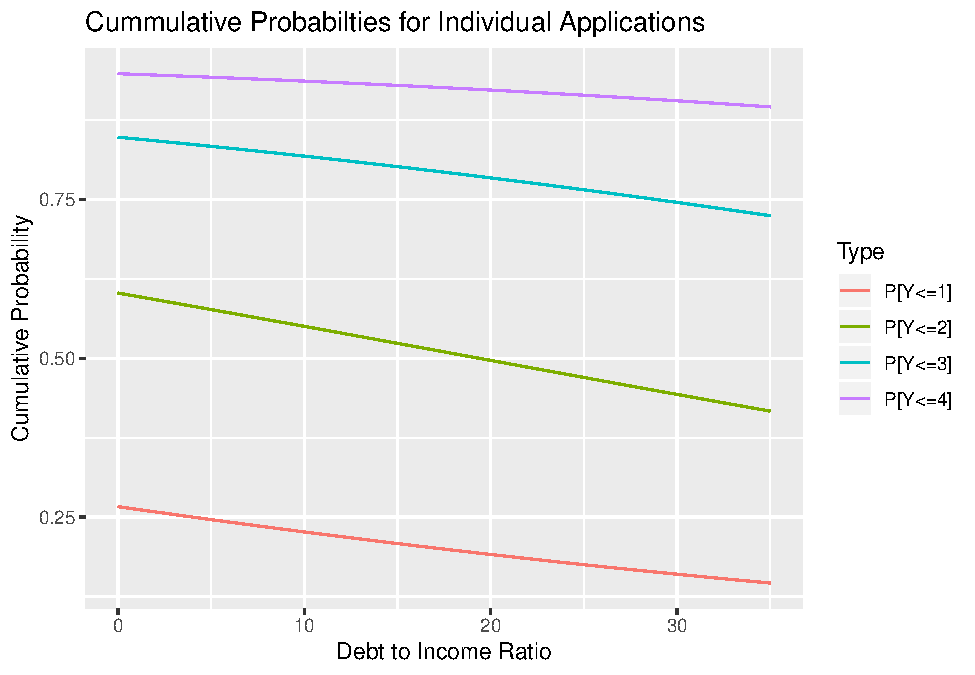
\includegraphics{SL_HW_5_files/figure-latex/unnamed-chunk-10-1.pdf}

The model above is a better fit than before, where lstat and crim seemed
to have a non-linear relationship with medv. adding an exponent to rm
seemed to improve fit, but also may be a case of over-fitting, which we
want to avoid, so it was kept untouched.


\end{document}
